\label{dogs}
DOGS is an extension of the DOG system. The first 3 letters can be directly translated from danish to \textit{dynamic optimization of greens} and the appended S of the herein regarded system means \textit{coordination}. Thus DOG is an traffic actuated optimizer for single intersections, as described in section \ref{actuated}, and DOGS add coordination.

DOGS is a criteria-based system which relies on a common cycle time for coordination. The intended area of application is traffic signals along arterials, which see a high fluctuation in demand. 

The DRD has implemented DOGS along several arterials in Denmark. 
Among these are the Glostrup and Herlev implementations along the important O3 ring-road. They see high increases in demand in the morning and afternoons with commuters. Normally such fluctuations can be handled well by a small number of timing plans (see section \ref{pretimed}), which are changed according to the time of day, but the area also see more unpredictable types of fluctuations when accidents occur on the nearby highway, M3, or when M3 lanes are closed due to expansions. For these reasons DRD decided implement a system which could handle such situations.

The purpose of DOGS is to increase the capacity of the arterial in the above mentioned cases and revert to offline-optimized, pretimed plans in low traffic situations. The capacity increase comes by increasing the common cycle time and allocate the extra green time per cycle to the phases along the arterial. This will cause increased delays for the minor roads, but may prevent queues from reaching the previous intersection - or even prevent queues in cases of light congestion.
DOGS is also capable of providing priority to buses by extending the green time when buses are near an intersection.

At present the system must be tailored to the environment in which it operates. For this reason the following sections will use the Herlev area as a reference area in order to explain certain concepts. In Figure \ref{fig:dogs_herlev} is a layout of this network.

\begin{figure}[!ht]
\begin{center}
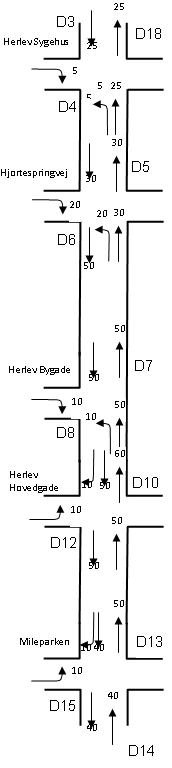
\includegraphics[scale=0.5]{dogs_herlev.png} 
\end{center}
\caption{Layout of the partial O3 arterial in Herlev, which is under DOGS control. The arrows and numbers indicate flow direction and examples of typical vehicle count.}
\label{fig:dogs_herlev}
\end{figure}

\subsubsection*{Detection}
Loops are placed in the immediate downstream of intersections and connected to closest controller to reduce the wire length. 

The criteria, which DOGS use, are based on the total inflow and outflow per cycle as well as load percentage, which, in Herlev, is extracted from strategically placed detectors in the ends of the arterial. In Figure \ref{fig:dogs_herlev} the inflow is thus measured at D3 and D14 while the outflow is measured at D15 and D18. 
During an interview with DRD and TTS it was explained that the traffic from minor roads can be neglected in the load measurement, though both parties would be interested in seeing the effect of increasing the number of detectors used.

In addition to vehicles per cycle and load degrees the detectors are capable of measuring vehicle speeds, though this is not taken into consideration in any of the criteria. In the case of prediction such capabilities could be taken advantage off eg. by fitting the predicted speeds to observations.
Individual vehicle speeds measured at detectors are usually not taken into consideration when performing prediction since they represent the speed at a single point rather than some average speed. It is possible that the average speeds measured at detectors can be used to estimate the level of congestion of the network as an alternative to travel time measurements by video.

\subsubsection*{Prediction}
DOGS is a purely traffic actuated system and no prediction is used when the system is activated due to heavy traffic conditions.

In spite of the intended flexibility of the system this is a point which puts high demand on the implementing traffic engineers since traffic through the arterial must be assessed manually when the system is put into production as well as during maintenance.

An alleviating point to the lack of prediction is the fact that the current arterials under DOGS control are relatively small and static predictions can be made by an experienced traffic engineer. Furthermore, since DOGS only operate under high load conditions, predictions become less valuable - or superfluous, even - because all that can be said about the arterial in this case is that it is heavily loaded with traffic.

\subsubsection*{Optimization}
Since DOGS only kicks in under congested or near-congested conditions (for the Herlev area when the load exceeds 60\%) it is simple to optimize the throughput since any increase in green time will just allow more vehicles to pass (the phase is never emptied from vehicles).

That DOGS only operates during high-congestion levels is an unusual trait for an adaptive system since they usually excel in optimization under \textit{normal} ie. uncongested load conditions (see the comparison of RHODES and a semi-actuated system in section \ref{rhodes}). This can be explained from the lack of an explicitly defined objective function and optimization routine.

The objective is to keep the load degree (load/capacity) for the most heavily loaded intersection below 90\%.
To do this the common cycle time and green times are set according to the load level. The adjustments are made with a few seconds per cycle to avoid sudden, major changes in cycle time and temporary loss of coordination.

Coordination is achieved by running the signals on a common cycle time, but offsets are not adjusted when the common cycle time changes so this issue should receive further investigation.

When naming the inflow detectors in the north- and south ends $DN$ and $DS$, respectively, the transition from pretimed control to adaptive control is decided by the constraint:
\begin{eqnarray*}
Intensity(DN) > I_{enable} & \vee & Intensity(DS) > I_{enable} \\
& or & \\
Load(DN) > L_{enable} & \vee & Load(DS) > L_{enable}
\end{eqnarray*}

For switching back to pretimed control this constraint must hold:
\begin{eqnarray*}
Intensity(DN) < I_{disable} & \wedge & Intensity(DS) < I_{disable} \\
& and & \\
Load(DN) < L_{disable} & \wedge & Load(DS) < L_{disable}
\end{eqnarray*}

To avoid hysteresis ie. constant enabling and disabling of dynamic control:
\begin{eqnarray}
I_{enable} - I_{disable} & \geq & I_{\varepsilon} \label{eqn:hysteresis_intensity} \\ 
L_{enable} - L_{disable} & \geq & L_{\varepsilon} \label{eqn:hysteresis_load} \\
I_{\varepsilon},L_{\varepsilon} & > & 0 \label{eqn:hysteresis_limits}
\label{eqn:hysteresis}
\end{eqnarray}

DOGS exhibits a dynamic behaviour because the permitted cycle time extensions are divided into \textit{programs} according to the intensity and load levels in the ends of the artery. These program constraints take a form which is similar to the enable- and disable constraints.

When deciding whether to remain in the current program, $i-1$, or switch to a program for higher demand, $i$, the following relation must be satisfied:

\begin{eqnarray*}
I_{enable,i+1} \geq & \max(Intensity(DN),Intensity(DS)) & > I_{enable,i} \\
& \vee & \\
L_{enable,i+1} \geq & \max(Load(DN),Load(DS))  & > L_{enable,i}
\end{eqnarray*}

The decision of switching from program $i$ to the program for lower demand, $i-1$, is determined by this relation:

\begin{eqnarray*}
I_{disable,i-1} \leq & \max(Intensity(DN),Intensity(DS)) & < I_{disable,i} \\
& \wedge & \\
L_{disable,i-1} \leq & \max(Load(DN),Load(DS))  & < L_{disable,i}
\end{eqnarray*}

In the DOGS controlled area in Herlev there are 8 different programs to choose from and the enable and disable thresholds for programs respect the ordering implicit in the above equations:

$$\lbrace I,L \rbrace_{enable,i+1} > \lbrace I,L \rbrace_{enable,i}$$
$$\lbrace I,L \rbrace_{disable,i-1} < \lbrace I,L \rbrace_{disable,i}$$

To avoid hysteresis between programs the same constraints (equations \ref{eqn:hysteresis_intensity}-\ref{eqn:hysteresis_limits}) as for switching between pretimed and dynamic control applies.

\subsubsection*{Evaluation}
Tests have shown that the system is indeed capable of increasing the capacity, with reduced queue lengths as a result. When the arterial in Herlev is at or above moderate load DOGS will increase the capacity by 15-25\% compared to the capacity if only the pretimed plans was in use.

Due to its ad-hoc nature it is difficult to compare DOGS to other systems for arterial progression. In a future project by this author simulations of DOGS will allow further comparison studies.